Die Geschwindigkeit ist die Steigung des $s(t)$-Graphen, nicht seine Höhe.
\begin{abcliste}
\abc Von \SI{0}{\second} bis \tOneO\ fällt der Graph: $\result{v<0}$. Von \tOneO\ bis \tTwoO\ ist er waagrecht: $\result{v=0}$, der Körper ruht. Von \tTwoO\ bis \tEndO\ steigt er: $\result{v>0}$.

\abc Die Stücke sind Geraden, die Geschwindigkeit ist darin konstant:
\begin{align}
 v_1 &= \vOneF = \frac{\sOne-\sNull}{\tOne} = \vOne \approx \result{\vOneP{0}{1}} \\
 v_3 &= \vThreeF = \frac{\sEnd-\left(\sOne\right)}{\tEnd-\tTwo} = \vThree \approx \result{\vThreeP{0}{2}}
\end{align}
Das $v(t)$-Diagramm:
\begin{center}
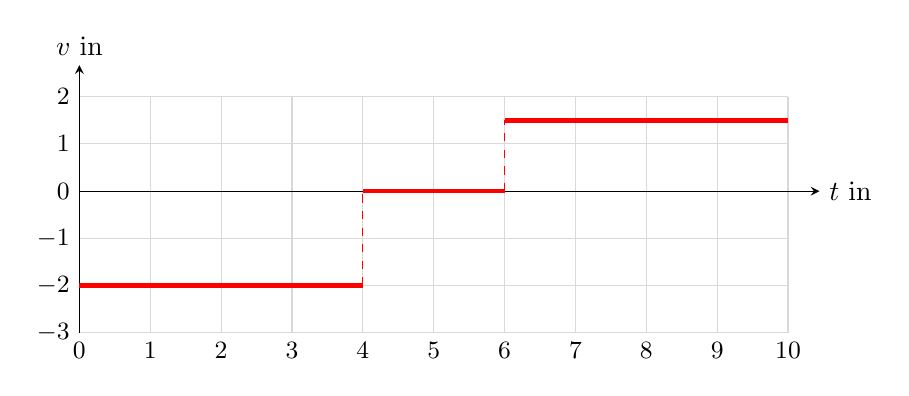
\begin{tikzpicture}[>=stealth, x=0.9cm, y=0.6cm]
 \draw[gray!30] (0,-3) grid[xstep=1, ystep=1] (10,2);
 \draw[->] (0,0) -- (10.444,0) node[right] {$t$ in \si{\second}};
 \draw[->] (0,-3) -- (0,2.667) node[above] {$v$ in \si{\meter\per\second}};
 \foreach \tk in {0,1,2,3,4,5,6,7,8,9,10} \node[below] at (\tk,-3) {\small $\tk$};
 \foreach \yk in {-3,-2,-1,0,1,2} \node[left] at (0,\yk) {\small $\yk$};

 \draw[ultra thick, red] (0,-2) -- (4,-2);
 \draw[ultra thick, red] (4,0) -- (6,0);
 \draw[ultra thick, red] (6,1.5) -- (10,1.5);
 \draw[red, dashed] (4,-2) -- (4,0) (6,0) -- (6,1.5);
\end{tikzpicture}
\end{center}
\abc Mia verwechselt den Ort mit der Geschwindigkeit. Dass $s$ negativ ist, sagt nur, dass der Körper auf der negativen Seite des Nullpunkts ist. Ab \tTwoO\ wird $s$ grösser ($-2$, $-1.25$, $-0.5$, \ldots), der Körper bewegt sich also in die positive Richtung: $\result{v = \vThreeP{0}{2} > 0}$, auch solange $s<0$ ist. Bei
\begin{align}
 t &= \tZeroF = \tZero \approx \tZeroP{0}{2}
\end{align}
fährt er durch den Nullpunkt, ohne dass sich seine Geschwindigkeit ändert. Umgekehrt ist die Geschwindigkeit von \SI{0}{\second} bis \SI{3}{\second} negativ, obwohl der Körper dort im positiven Bereich ist.
\end{abcliste}
